\documentclass[letterpaper, 10pt, conference]{ieeeconf}
\usepackage{times}


\IEEEoverridecommandlockouts 
\overrideIEEEmargins


\usepackage{cite}
\usepackage{graphicx}     
\usepackage{amssymb,amsmath}
\usepackage{algorithm}
\usepackage[noend]{algorithmic}
\usepackage{flushend}
\usepackage[export]{adjustbox}
\renewcommand{\thefootnote}{\fnsymbol{footnote}}

\newcommand{\Acronym}[1]{\ensuremath{{\small{\texttt{#1}}}}}
\newcommand{\Symbol}[1]{\ensuremath{\mathcal{#1}}}
\newcommand{\Function}[1]{\ensuremath{{\small \textsc{#1}}}}
\newcommand{\Constant}[1]{\ensuremath{\small{\texttt{#1}}}}
\newcommand{\Var}[1]{\ensuremath{{\small{\textsl{#1}}}}}
\newcommand{\False}{\Constant{false}}
\newcommand{\True}{\Constant{true}}
\newcommand{\Null}{\Constant{null}}
\newcommand{\Name}{\Acronym{dCRoPS}}
\newcommand{\Revision}[1]{\textcolor{red}{#1}}
\newcommand{\R}{\ensuremath{\mathbb{R}}}
\newcommand{\Traj}{\ensuremath{\zeta}}
\newcommand{\Tree}{\Symbol{T}}

%\setlength{\abovedisplayskip}{1pt}
%\setlength{\belowdisplayskip}{1pt}

\begin{document}

\title{Path Planning for Swarms in Dynamic Environments by\\ Combining Probabilistic Roadmaps and
  Potential Fields}


\author{Alex Wallar \and Christopher Choi \and Erion Plaku
\thanks{A. Wallar and C. Choi are with the School of Computer Science,
  University of St Andrews, Fife KY16 9AJ, Scotland, UK. E. Plaku is with the
  Dept. of Electrical Engineering and Computer Science, Catholic
  University of America, Washington DC 20064 USA.
}}


\maketitle
\begin{abstract}
This paper presents a path-planning approach to enable a swarm of
robots move to a goal region while avoiding collisions with static and
dynamic obstacles.  To provide scalability and account for the
complexity of the interactions in the swarm, the proposed approach
combines probabilistic roadmaps with potential fields.  The underlying
idea is to provide the swarm with a series of intermediate goals which
are obtained by constructing and searching a roadmap of likely
collision-free pathways. As the swarm moves from one intermediate goal
to the next, it relies on potential fields to quickly react and avoid
collisions with static and dynamic obstacles. Potential fields are
also used to ensure that the swarm moves in cohesion. When the swarm
deviates or is unable to reach the planned intermediate goals due to
interferences from dynamic obstacles, the roadmap is searched again to
provide alternative pathways. Experiments conducted in simulation
demonstrate the efficiency and scalability of the approach.
\end{abstract}


\section{Introduction}
\label{sec:Intro}

Emerging applications of swarm robotics in exploration, monitoring,
inspection, and search-and-rescue missions require the swarm to be
able to move in cohesion to a goal destination while avoding
collisions with obstacles \cite{swarm,swarmReview12}.  As the swarm is
often comprised of a large number of robots, path planning becomes
challenging due to the high-dimensionality of the underlying
configuration space.

As a result, reactive approaches are often employed that avoid
planning directly in the high-dimensional configuration space but
instead regulate the swarm behavior through common rules of
interactions. Stigmergic approaches, inspired by how ants move
back-and-forth from the nest to a food source, utilize synthetic
pheromone traces left in the environment by forager robots to guide
the swarm to the target
\cite{swarmPheromone1,swarmPheromone2,swarmPheromone3}.  While
pheromone-based navigation minimizes communication, it lacks the
flexibility to quickly adapt to dynamic changes in the environment
that could block or disrupt existing pheromone traces. Other
approaches rely on wireless network nodes deployed at various
locations in the environment to provide global coverage and guide the
swarm to the target \cite{swarmComm1,swarmComm2}.  Genetic algorithms
have also been used to facilitate navigation by evolving collective
behaviors for the swarm, such as chain formation or obstacle avoidance
\cite{swarmEvolve1,swarmEvolve2}.  In leader-follower approaches, one
or few robots move along precomputed paths to the target location
while the rest of the swarm seeks to follow the leaders, often
maintaining a desired formation
\cite{swarmLeader1,swarmLeader2,swarmLeader3}. The work in
\cite{JurVel} proposes a fully-decentralized algorithm based on
the concept of reciprocal velocity obstacles to enable collision-free
motions among a group of robots. Other approaches based
on virtual fixtures treat the swarm as a rigid body, seeking to
maintain a fixed relation among swarm members
\cite{swarmFixture1,swarmFixture2,swarmFixture3}. While such
approaches reduce swarm path planning to single-robot planning, the
imposed structure rigidity and the increased dimensionality make it
difficult to efficiently plan paths especially when considering a
large number of robots. 


Artificial potential functions (APFs) provide a common approach for
swarm path planning by imposing virtual repulsive forces from
obstacles and attractive forces to the goal
\cite{Khatib86,reif1999social,book:SwarmsAPFs,tanner2005formation,swarmPF1,swarmPF2}.
APFs are fast to compute as the resulting forces for each robot in the
swarm depend only on the nearby obstacles, the goal region, and
limited interactions with neighboring robots in the swarm.  While APFs
provide local, reactive, behaviors that enable the swarm to avoid
obstacles, the global path guidance toward the goal suffers from local
minima.  This limitation of APFs becomes more prevalent when
considering path planning for large swarms moving in cluttered
environments. Designing APFs that avoid or minimize the likelihood of
the robots becoming stuck in local minima remains a challenging problem
\cite{RK92}.

Alternative approaches seek to avoid local minima by relying on global
path planning. Probabilistic roadmaps (PRM) \cite{PRM} and other
sampling-based path planners
\cite{RRT,RRTRecent1,TogglePRM,UOBPRM,PlakuTRO10} provide global path
planning by using sampling to capture the connectivity of the free
configuration space. In particular, PRM approaches construct roadmaps
resembling a network of roads obtained by sampling a large number of
configurations and connecting neighboring configurations via
collision-free paths.  The roadmap is then used to perform different
tasks, such as homing, goal searching, or shepherding
\cite{LienSwarming,LienShepherding}.  PRMs have also been combined
with Bezier curves to guide a number of nonholonomic robots to the
goal while maintaining formation \cite{KostasSwarm}.

While PRMs avoids the issues associated with local minima, scalability
starts becoming problematic when dealing with a large number of
robots. As the configuration space of a swarm consist of the Cartesian
product of the individual configuration spaces of each robot, it
becomes challenging to generate collision-free configurations and
connect neighboring configurations via collision-free paths. 
 
To provide scalability and account for the complexity of the
interactions in the swarm, this paper builds upon our prior work
\cite{PlakuTAROS13boids} which combined PRMs with APFs. While prior
work was limited to static obstacles, the proposed approach, termed
$\Name$ (\texttt{C}ombined \texttt{Ro}admaps and \texttt{P}otentials
for \texttt{S}warms for \texttt{D}ynamic Obstacles), can efficiently
guide the swarm to the goal even in the presence of dynamic obstacles.
The underlying idea is to provide the swarm with a series of
intermediate goals which are obtained by constructing and searching a
roadmap of likely collision-free pathways. To maintain scalability,
the roadmap is constructed over the two-dimensional workspace in which
the swarm moves rather than the high-dimensional configuration space
associated with the swarm. As the swarm moves from one intermediate
goal to the next, it relies on potential fields to quickly react and
avoid collisions with static and dynamic obstacles. In contrast to
prior work \cite{PlakuTAROS13boids}, $\Name$ introduces the idea of
branching, which provides robots in the swarm with alternative
pathways to the goal when a robot  is
unable to reach the planned intermediate goals due to interferences
from dynamic obstacles. Weights of roadmap vertices and
edges in or near the obstructed area are dynamically adjusted to
account for lack of progress and to guide the swarm away from such
areas. $\Name$ also improves the APFs in order to enable the swarm to
react rapidly to dynamic obstacles moving towards it.
Experiments are conducted in simulation where large
swarms have to move in complex environments, often through narrow
passages, while avoiding collisions with static obstacles and numerous
dynamic obstacles. Results demonstrate the efficiency and scalability
of $\Name$.

\section{Problem Formulation}
\label{sec:Problem}
The swarm consists of a number of mobile circular robots $b_1, \ldots,
b_n$ operating in a two-dimensional workspace $W$.  Each robot
is capable of detecting nearby obstacles.  Starting at an initial
placement, the objective is for each robot to reach a goal
region $G \subset W$ while avoiding collisions with static and dynamic
obstacles present in the workspace $W$. While branching is allowed, $\Name$ seeks to keep the
robots moving as a swarm as much as possible, branching off only when
necessary to avoid dynamic obstacles. The geometry and placement of each static obstacle is
assumed to be available beforehand. No information is given to $\Name$
in regards to the dynamic obstacles. 

\section{Method}
\label{sec:Method}

Pseudocode for $\Name$ is provided in Algorithm~\ref{algo}. The
main steps are described below.


\subsection{Global Path Planning}

As mentioned, $\Name$ uses a roadmap to provide the swarm with global
path planning and find alternative pathways to the goal when dynamic obstacles
prevent the swarm from moving along the current pathway. 

\subsubsection{Roadmap Construction}
The roadmap is represented as a graph $RM=(V,E)$. A vertex $q \in V$
corresponds to a collision-free point in the workspace. An edge $(q_i,
q_j) \in E$ corresponds to a collision-free path from $q_i$ to $q_j$.
Collision checking during roadmap construction is performed with
respect to the static obstacles, which are assumed to be known.  The
roadmap is later repaired in response to interference by dynamic
obstacles.


\begin{algorithm}[t]
\caption{Pseudocode for $\Name$}
\label{algo}
\begin{algorithmic}[1]
\setcounter{ALC@line}{0}
%\COMMENT{generate $n$ additional roadmap vertices}
\vspace*{1mm}
\STATE $RM = (V, E) \leftarrow \Function{ConstructRoadmap}()$
\STATE $w(q_i) \leftarrow$ assign weight to each vertex $q_i \in V$
\STATE $w(q_i, q_j) \leftarrow$ assign weight to each edge $(q_i, q_j) \in E$
\STATE $\zeta = [q_k]_{k=1}^m \leftarrow
\Function{pathway}(RM, [w(q_i)], [w(q_i, q_j)])$
\STATE \textbf{for} $b \in \Var{Robots}$ \textbf{do}
$\Var{goal}_b\leftarrow \zeta(1)$; $\Var{pathway}_b \leftarrow \zeta$
\WHILE{$\Function{solved}() = \False$}
\FOR{$b \in \Var{Robots}$ \textbf{with}
$\Function{reached}(b, \Var{goal}_b) = \True$} 
\STATE $\Var{goal}_b \leftarrow \Function{NextGoal}(\Var{pathway}_b, b)$
\ENDFOR
\FOR{$b \in \Var{Robots}$ \textbf{with}
$\Function{stuck}(b) = \True$} 
\STATE $\Var{pathway}_b \leftarrow \Function{branching}(RM, [w(q_i)], [w(q_i,q_j)],b)$
\STATE $\Var{goal}_b \leftarrow \Var{pathway}_b(1)$
\ENDFOR


\FOR{$b \in \Var{Robots}$ }
\STATE $\Var{pf}_b \leftarrow \Function{superimpose}(PF_\Var{obst}(b),
PF_\Var{sep}(b),$\\ \hfill{$PF_\Var{goal}(b),PF_\Var{heading}(b))$}
\ENDFOR

\FOR{$b \in \Var{Robots}$ }
\STATE $\Var{heading}_b \leftarrow w_1 \Var{heading}_b + w_2 \Var{pf}_b$
\STATE $\Var{pos}_b \leftarrow \Var{pos}_b + \Var{heading}_b$
\ENDFOR
\ENDWHILE


\end{algorithmic}
\end{algorithm}

In order to avoid cluttered or narrow-passage areas, which are more
likely to lead to collisions with dynamic obstacles, $\Name$
generates roadmaps vertices that are at least a certain
distance, $d_\Var{clear}$, away from the static obstacles.
Each roadmap vertex is generated by sampling a point at random inside
the workspace $W$ until it
satisfies both of the above conditions.

A weight $w(q)$ is associated with each vertex $q \in V$ as an
estimate on the feasibility of the swarm to pass near $q$. More
specifically, $w(q)$ is defined as
$$
w(q) = (\sum_{o \in \Var{StaticObstacles}} \Var{dist}(q, o))^3,
$$
where $\Var{dist}(q, o)$ denotes the distance from the point $q$ to
the obstacle $o$. Small values of $w(q)$ are indicative of nearby
obstacles, which the swarm will seek to avoid. 
Note that while we have chosen
through experimentation a particular definition of $w(q)$ for this
paper, alternative weight functions can also be used.

Roadmap edges are generated by connecting each $q \in V$ to its
$k$-nearest roadmap vertices according to the Euclidean
distance. Collision checking is performed with respect to static
obstacles, discarding any edge that is found in collision. A weight
$w(q_i, q_j)$ is associated with each edge $(q_i, q_j) \in E$
as an estimate on the feasibility of having the swarm move from $q_i$
to $q_j$. More specifically, $w(q_i, q_j)$ is defined as 
$$
w(q_i, q_j) = ||q_i, q_j||_2 / \min(w(q_i), w(q_j)),
$$
As such, small values of $w(q_i, q_j)$ indicate that $q_i$ and $q_j$
are close to each other but away from obstacles.

\subsubsection{Guiding the Swarm}

A global pathway $\zeta = [q_i]_{i=1}^m$ (Algorithm~\ref{algo}:4)
guides the swarm to the goal region. The pathway is computed using
Dijkstra's algorithm to search the roadmap $RM=(V,E)$ for the shortest
path from start to goal. Such pathway, as a result of edge weights,
seeks to keep the swarm away from cluttered areas and narrow passages.
Initially, each robot $b$ is
given $\zeta$ as the pathway that it needs to follow
(Algorithm~\ref{algo}:5). The objective for each robot is to move to
$\Var{area}(\zeta(1)), \ldots, \Var{area}(\zeta(m))$ in succession,
where $\Var{area}(q)$ denotes a small area around $q$ (defined as a
disk with radius $d_\Var{clear}$). As discussed later in the section,
an attractive potential is used to move $b$ from its current position
to the next goal area along the pathway $\zeta$ (Algorithm~\ref{algo}:7--8).

\subsubsection{Branching} 

If a robot $b$ gets stuck in a local minima or a dynamic obstacle
prevents it from reaching its next target $\Var{area}(q_i)$ along its
current pathway, $\Name$ will search the roadmap again to find an
alternative pathway for $b$ (Algorithm~\ref{algo}:9--10).  Before the
roadmap search, $\Name$ adjusts the weight of the next few edges
$(q_i, q_{i+1}), (q_{i+1}, q_{i+2}), \ldots, (q_{i+\ell -1},
  q_{i+\ell})$ on the current path in order to guide $b$ away from
  this area.  This local repair is used to relieve swarm congestion
  when it is confronted by an obstructing obstacle. The creation of a
  new pathway may not always make the swarm move faster to the end
  goal, but it reduces the average wait time, the average time stuck,
  and it can guide the swarm around obstructing dynamic obstacles that
  are blocking critical passageways.

\subsection{Local Path Planning}
$\Name$ uses APFs to make the swarm follow the current global
pathway and quickly react to obstacles it may encounter along the way.
Several criteria are taken into consideration when designing
the APFs for a robot $b$:
\begin{enumerate}
\item $b$ is attracted to its next goal; 
\item $b$ is repulsed away from obstacles; 
\item $b$ seeks to move in cohesion with its neighbors without
  straying too far away or getting too close.
\end{enumerate}

\subsubsection{Attraction to the Next Goal}

Let $\Var{goal}_b$ denote the next goal for the robot $b$. To pull the
robot to the goal, $\Name$ defines an attractive potential as follows:
$$
PF_\Var{goal}(b) = \frac{\Var{goal}_b - \Var{pos}_b}{1 +
  \exp(\delta_\Var{goal}\, ||\Var{goal}_b, \Var{pos}_b||_2)},
$$ where $\delta_\Var{goal}$ is a scaling constant. Although stronger
potentials could be defined, using a weaker potential
enables the robot to reach $\Var{goal}_b$ while allowing for other behaviors
(such as obstacle avoidance) to take priority. When $\Var{goal}_b$ is
reached, the next goal along $\Var{pathway}_b$ is set as the target 
for $b$.


\subsubsection{Repulsion from Obstacles}
\label{sec:PFobst} 
To avoid collisions, $\Name$ relies on a repulsive potential to push
each robot away from the obstacles. Since $\Name$ is  
designed for dynamic obstacles, the responsiveness in the
obstacle potential needs to also increase in order for the
robots to react quickly to moving obstacles. More specifically, 
the repulsive potential between a robot $b$ and an obstacle $o$ is
defined as
$$ 
PF_\Var{obst}(b, o) = \frac{\Var{pos}_b
- \Var{ClosestPoint}(o, \Var{pos}_b)}{\sqrt{\vert(\Var{dist}(\Var{pos}_b, o) - \Var{radius}_b)\vert}}.
$$
As it is common in APFs, obstacles that are far away do not exert any
repulsive forces. As such, only obstacles that are within a certain
distance $\Delta_\Var{obst}$ from $\Var{pos}_b$ are used for the
computation of the overall repulsive potential, i.e.,
$$
PF_\Var{obst}(b) = \sum_{\stackrel{o \in
    \Var{Obstacles}}{\Var{dist}(\Var{pos}_b, o) \leq \Delta_\Var{obst}}}  PF_\Var{obst}(b, o).
$$

\subsubsection{Moving in Cohesion with Neighbors}

In order to ensure that robots do not get too close to one another,
which could lead to collisions and swarm congestion, $\Name$ imposes a
repulsive potential. A weak potential is used instead of a strong one
as the objective is to push $b$ at a safe distance from its neighbors
but not to separate it from the swarm. For this reason, the repulsive
potential between two robots $b_i$ and $b_j$ is defined as
$$
PF_\Var{sep}(b_i, b_j) = \frac{pos_{b_i}-pos_{b_j}}{1 +
  \exp(\delta_\Var{sep}\, ||\Var{pos}_{b_i}, \Var{pos}_{b_j}||_2)},
$$
where $\delta_\Var{sep}$ is a scaling constant. Similar to the case of
the repulsive potential for obstacles, only robots that are within a
certain distance $\Delta_\Var{sep}$ have an influence on $b$, i.e.,
$$
PF_\Var{sep}(b) = \sum_{\stackrel{b_i \in
    \Var{Robots} - \{b\}}{\Var{dist}(b, b_i) \leq \Delta_\Var{sep}}}  PF_\Var{sep}(b, b_i).
$$
In order to make the robots move in cohesion, the heading of the neighbors also exert an
influence on $b$. Preference is given to neighbors that
are not stuck (as such neighbors can help $b$ avoid
obstacles), and are neither too far nor too close to $b$.
More specifically, the potential function is defined as
$$
PF_\Var{heading}(b) = \sum_{b_i \in
    \Var{Neighs}(b)} \Var{heading}_{b_i},
$$
where $\Var{Neighs}(b)$ are selected as the $k$-closest nonstuck
robots to $b$ according to 
$$
\gamma(b, b_i) = \exp\left(\frac{-(||\Var{pos}_b, \Var{pos}_{b_i}||_2 - \mu)^2}
{2\sigma^2}\right),
$$
where $\gamma(b, b_i)$ is a Gaussian function with mean $\mu$ and
standard deviation $\sigma$.

\subsection{Combining the Potential Fields}
The overall effect on $b$ is obtained by combining the four different
potential fields: 
$$
PF(b) = \frac{\sum_{\phi \in \Var{fields}} \left(|| PF_\phi(b)||_2
  PF_\phi(b)\right)}{\sum_{\phi \in \Var{fields}} || PF_\phi(b)||_2},
$$
where $\Var{fields} = \{\Var{goal}, \Var{obst}, \Var{sep}, 
\Var{heading}\}$. This overall force is then used to update the
position and heading of $b$ (Algorithm~\ref{algo}:15--16).
In this way, $b$ is attracted to the next goal, strongly repulsed from
the obstacles, seeks to maintain a minimum separation distance from
its neighbors without getting separated from the swarm, and moves in
cohesion with its neighbors toward the next goal. When a robot becomes
stuck, the roadmap is locally repaired a new alternative pathway is
computed to help it escape. This combination of global path planning
via roadmaps and local path planning via potential fields enables the
approach to effectively guide the swarm to the final goal while
avoiding collisions with static and dynamic obstacles. 


\section{Experiments and Results}
\label{sec:ExpResults}

Experiments are conducted in simulation with an increasing number of
robots moving in complex environments, seeking to avoid numerous
static and dynamic obstacles. Results demonstrate the efficiency and scalability
of $\Name$.


\begin{figure*}
\centering
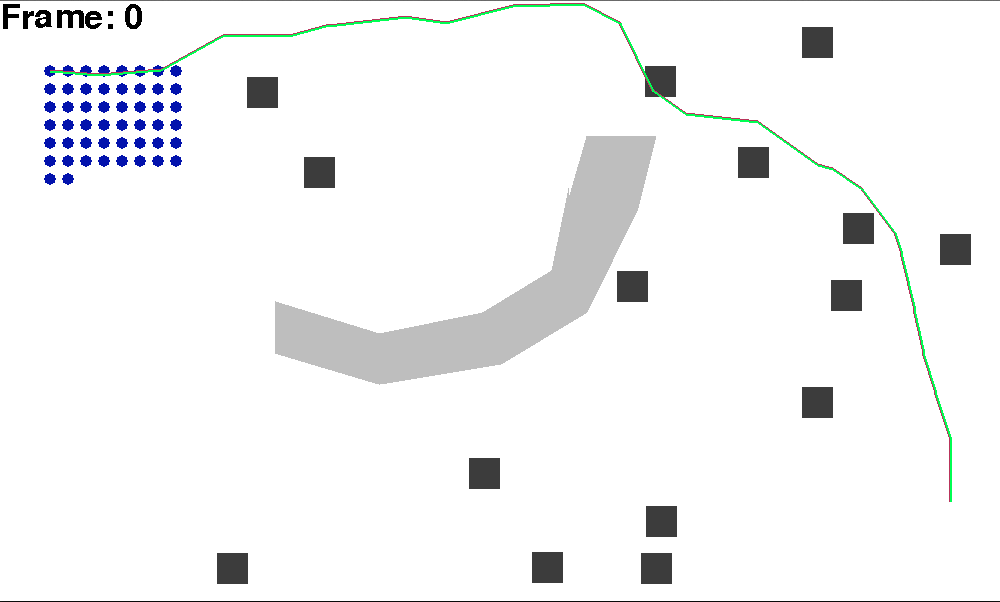
\includegraphics[width=0.24\textwidth,height=1.35in,frame]{figs/great_divide_1.png}
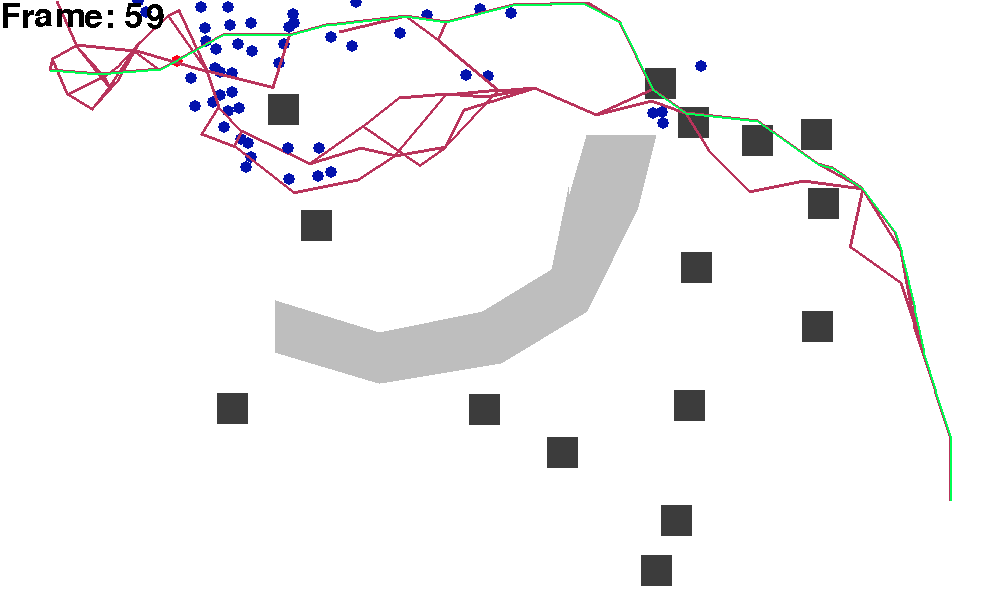
\includegraphics[width=0.24\textwidth,height=1.35in,frame]{figs/great_divide_2.png}
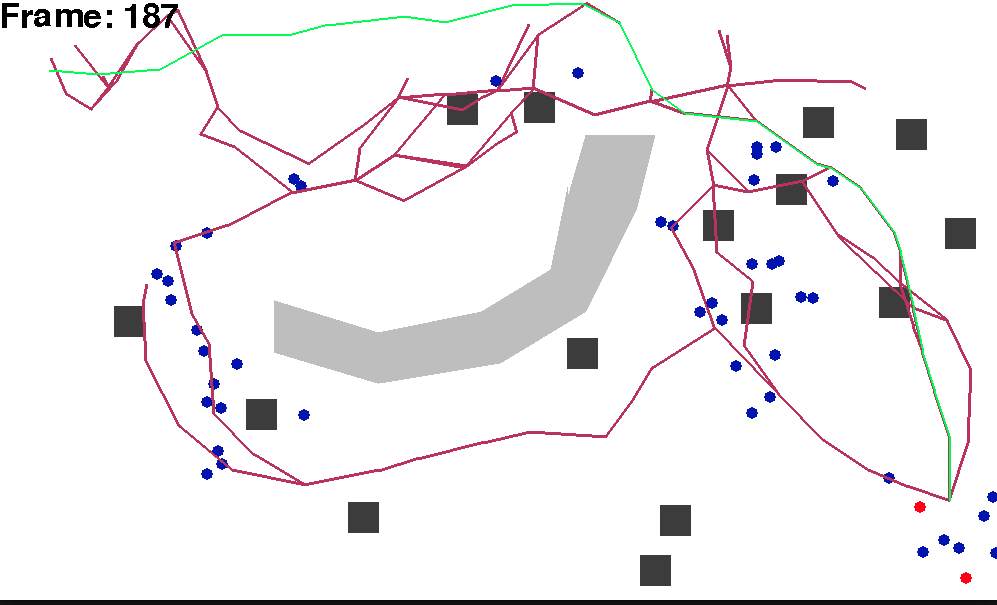
\includegraphics[width=0.24\textwidth,height=1.35in,frame]{figs/great_divide_3.png}
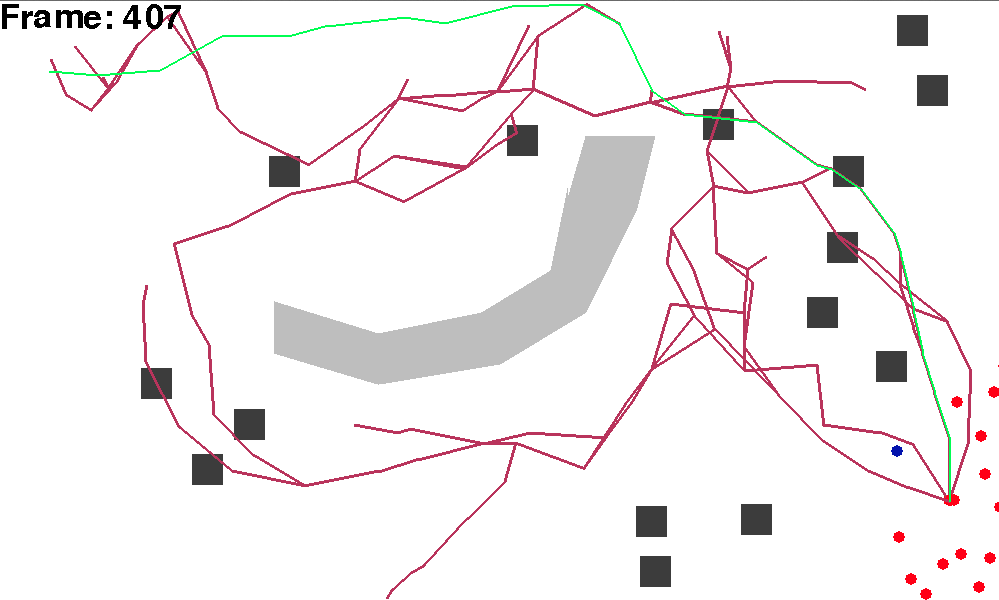
\includegraphics[width=0.24\textwidth,height=1.35in,frame]{figs/great_divide_4.png}\\[2mm]
(a) scene 1\\[2mm]
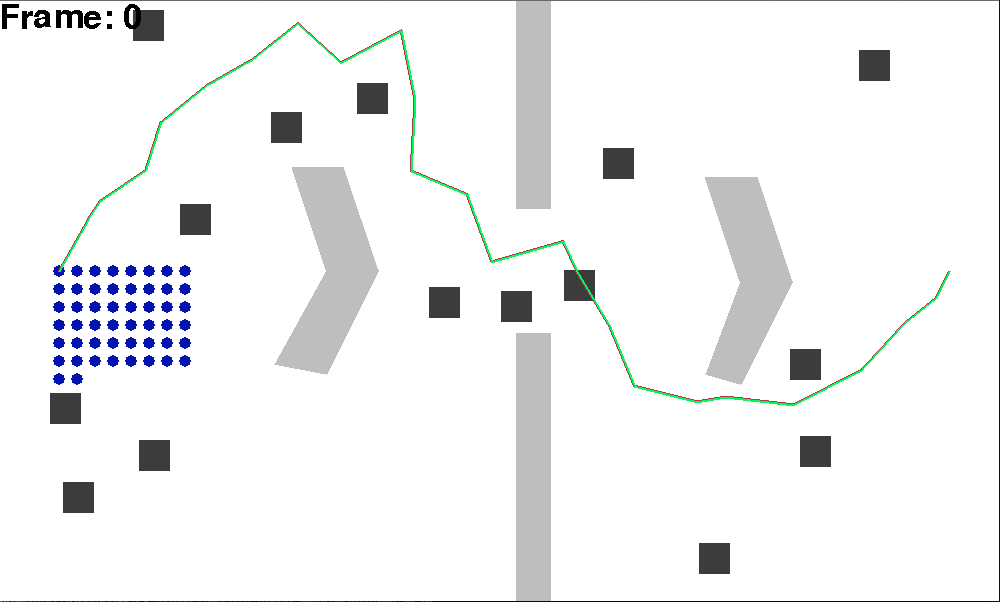
\includegraphics[width=0.24\textwidth,height=1.35in,frame]{figs/hurdles_1.png}
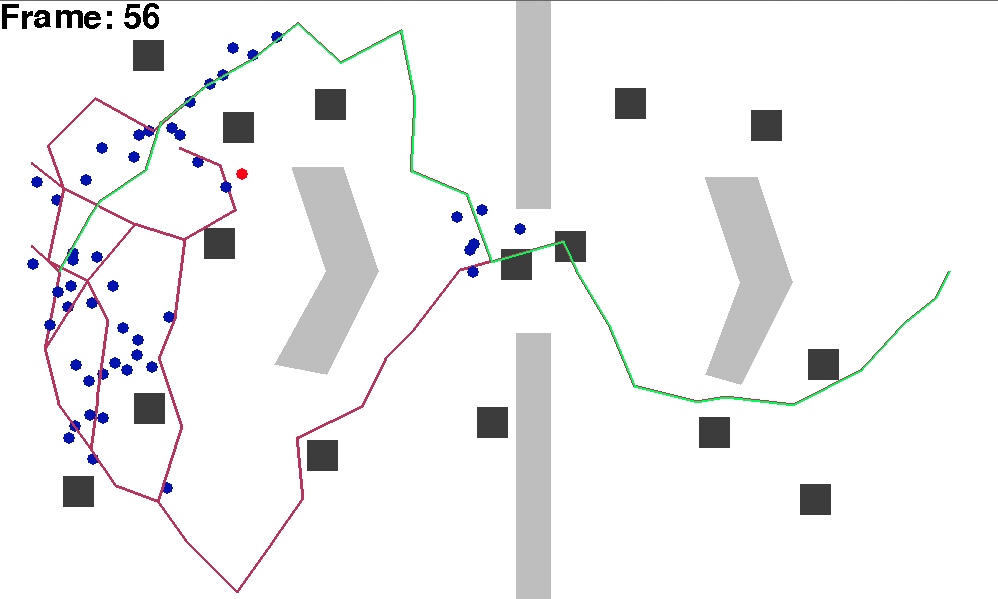
\includegraphics[width=0.24\textwidth,height=1.35in,frame]{figs/hurdles_2.png}
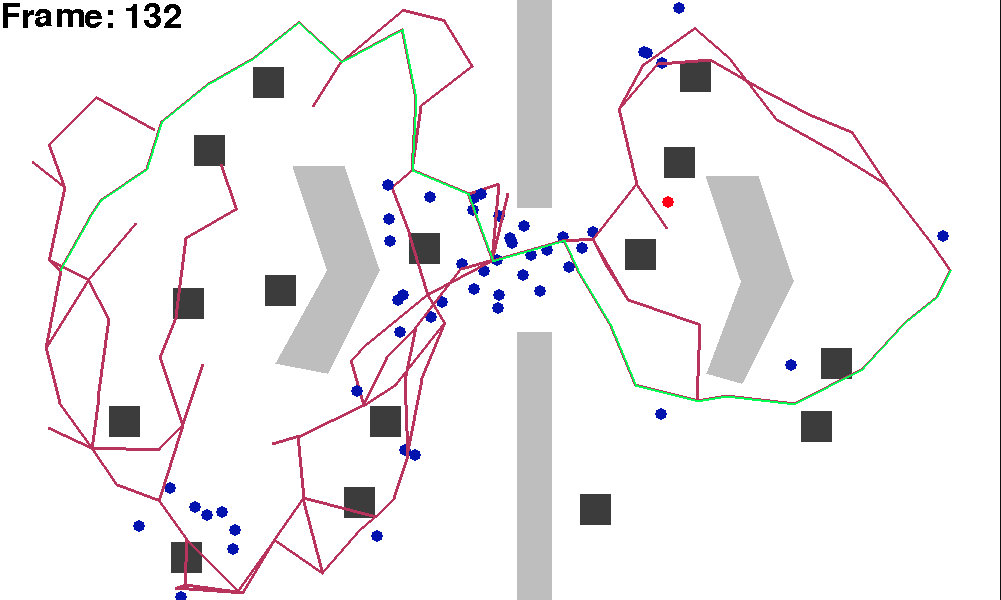
\includegraphics[width=0.24\textwidth,height=1.35in,frame]{figs/hurdles_3.png}
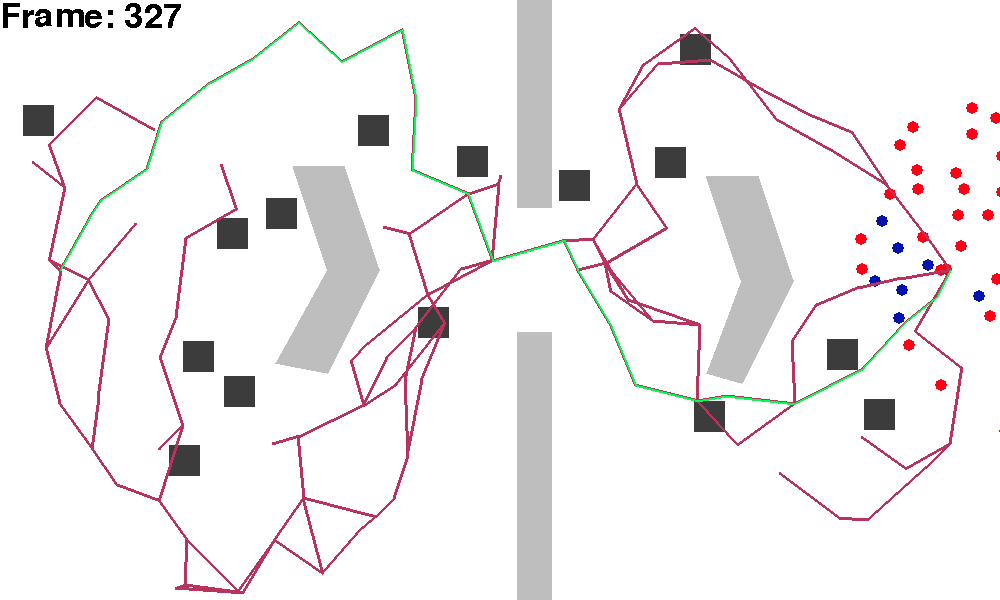
\includegraphics[width=0.24\textwidth,height=1.35in,frame]{figs/hurdles_4.png}\\[2mm]
(b) scene 2\\[2mm]
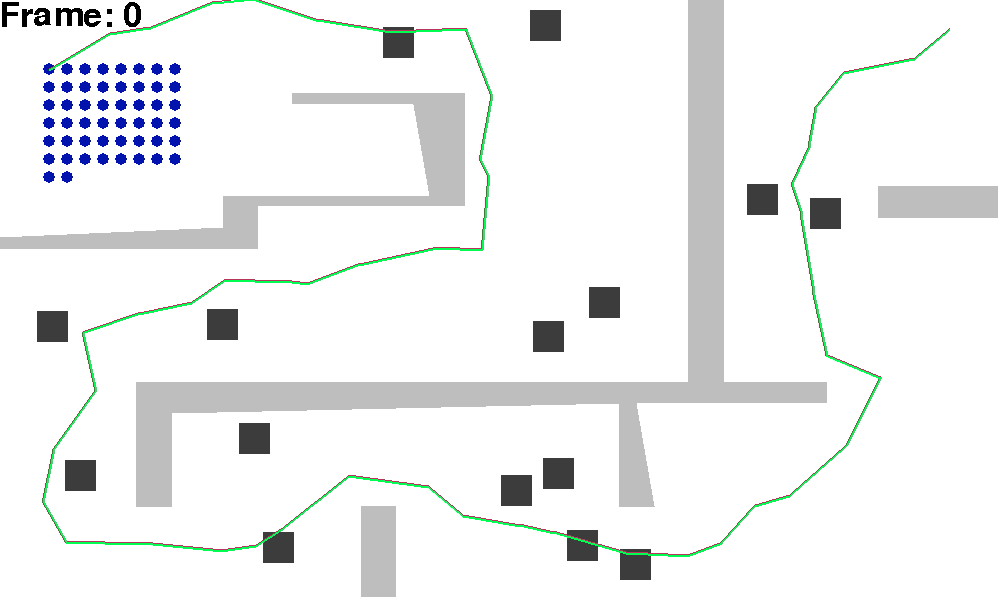
\includegraphics[width=0.24\textwidth,height=1.35in,frame]{figs/maze2_1.png}
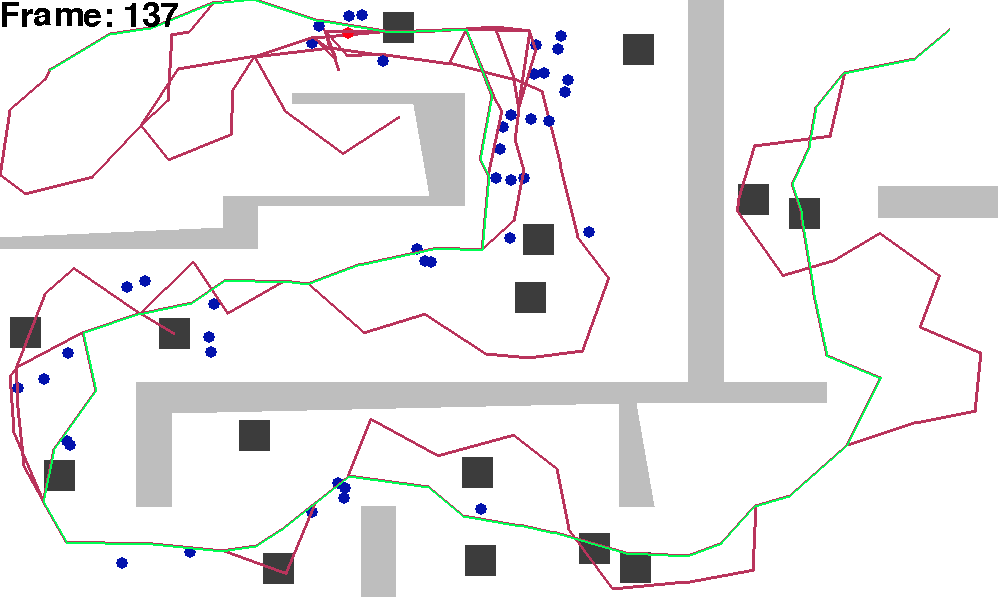
\includegraphics[width=0.24\textwidth,height=1.35in,frame]{figs/maze2_2.png}
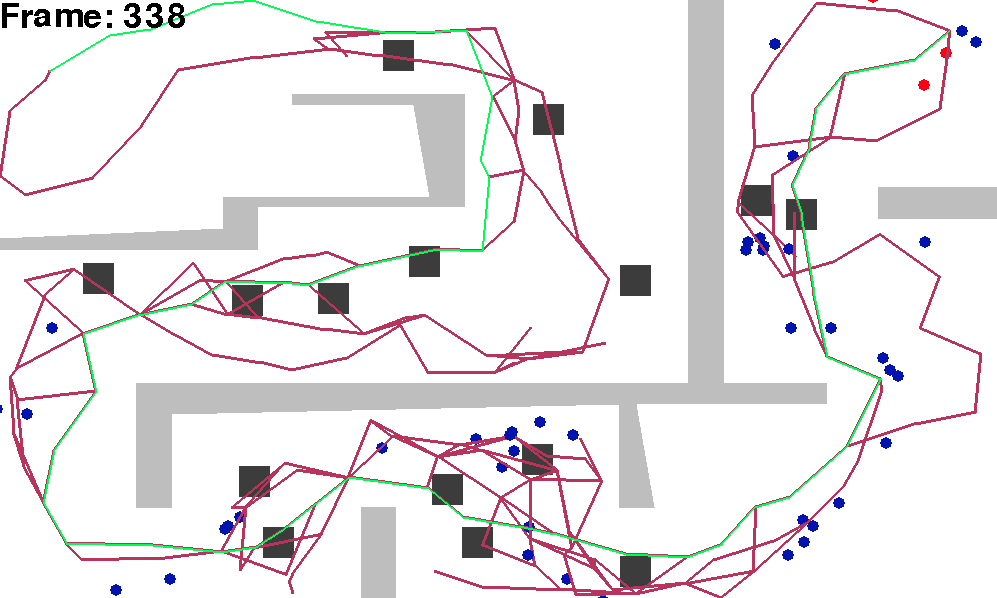
\includegraphics[width=0.24\textwidth,height=1.35in,frame]{figs/maze2_3.png}
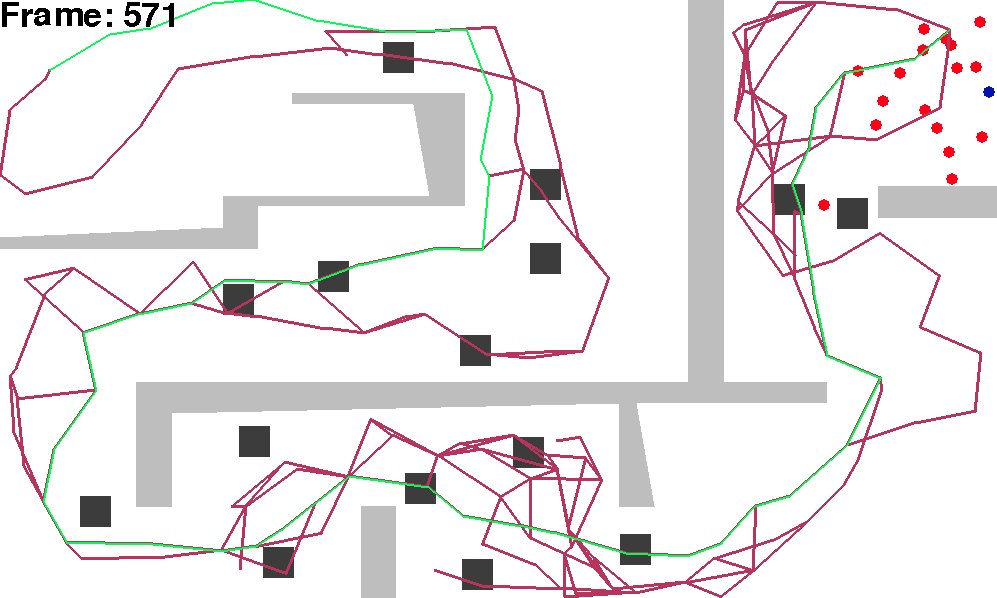
\includegraphics[width=0.24\textwidth,height=1.35in,frame]{figs/maze2_4.png}\\[2mm]
(c) scene 3
\caption{Illustration of $\Name$ on three different scenes. For each
  scene, four frames of a run of $\Name$ are shown. The first frame shows the
  swarm in the initial placement. The other three frames show how the
  swarm progresses towards the final goal. Static obstacles are shown
  in light gray. Dynamic obstacles are shown in dark grey. The initial
pathway is shown in green (see first frame). Alternative pathways that
are computed when some robots get stuck are shown in other colors.}
\label{fig:Scenes}
\end{figure*}


\subsection{Experimental Setup}

An illustration of the three different scenes used in the experiments
is provided in Fig.~\ref{fig:Scenes}. Each scene is comprised of
static and dynamic obstacles. These scenes provide challenging test
cases as the swarm has to go through numerous narrow passages that are
frequently blocked by dynamic obstacles. 


\subsubsection{Random Motions for the Dynamic Obstacles}
Recall that $\Name$ has no a
priori information on the behavior of the dynamic obstacles. In the
experiments, dynamic obstacles are made to move at random. More
specifically, they can only traverse in four directions, up, down,
left, or right. Each dynamic obstacle has a fixed change-direction
threshold that is triggered when the dynamic obstacle has
traveled along the current direction for a set distance. At that
point, the dynamic obstacle decides uniformly at random to go left,
right, up, or down. Robots have no influence on the direction or speed
of dynamic obstacles. When a dynamic obstacle encounters a static
obstacle, it starts traveling in the opposite direction.



\begin{figure*}
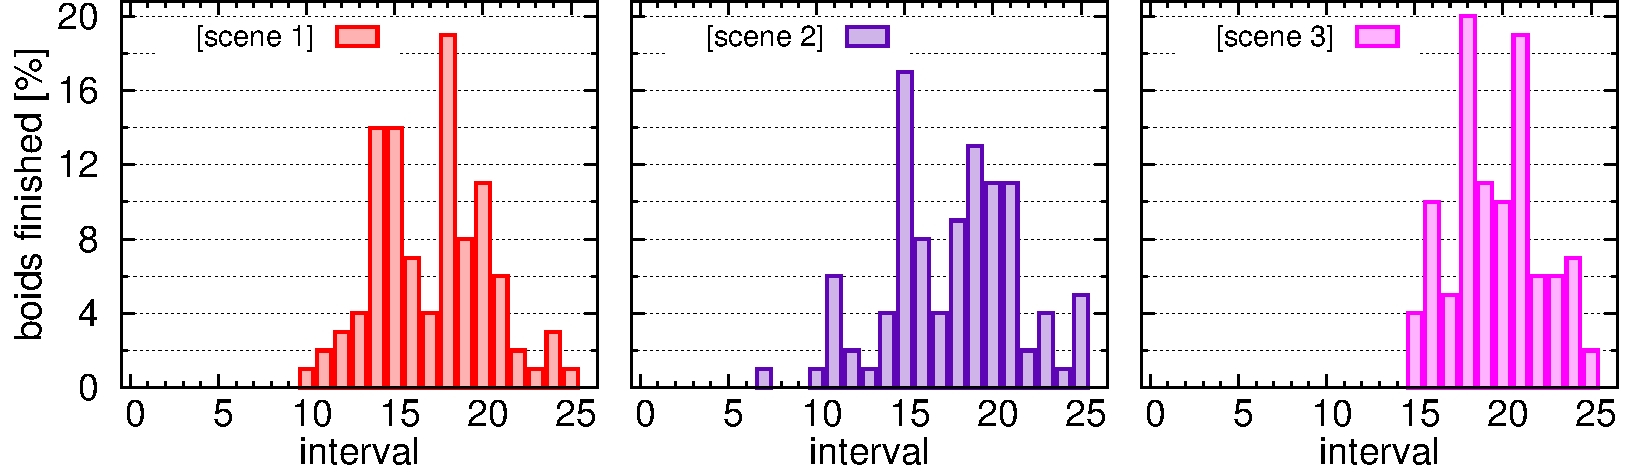
\includegraphics[width=\textwidth]{figs/figResHists}
\caption{Histogram on the time-to-reach final goal when running $\Name$ with
$100$ boids and $15$ dynamic obstacles on each of the scenes. In each
  case, the overall time is divided into $25$ equally-sized
  intervals. The $i$-th bar indicates the 
 percentage of robots that reached the final goal during the $i$-th time interval.}
\label{fig:Hist}
\end{figure*}


\begin{figure*}
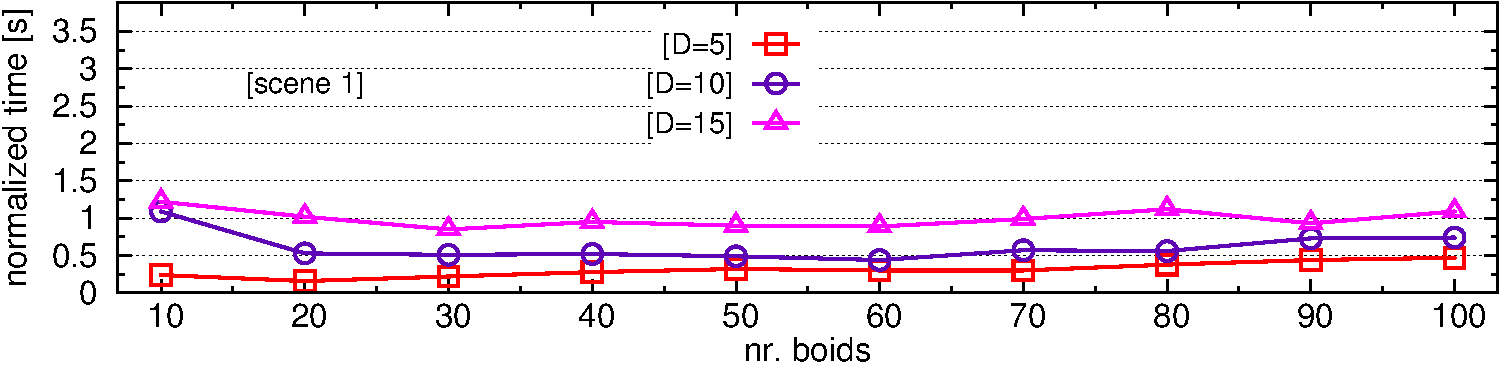
\includegraphics[width=\textwidth]{figs/figResScene1}\\
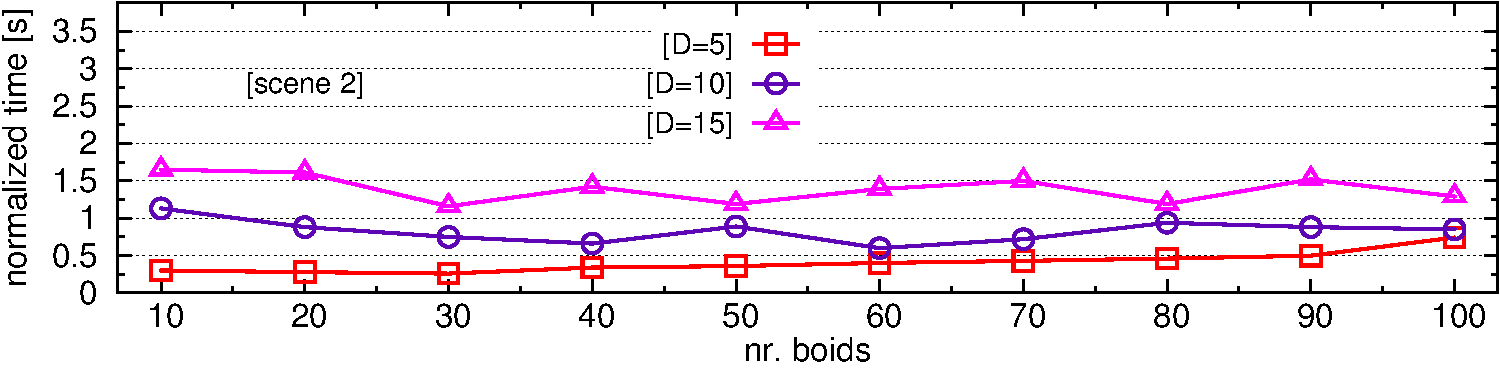
\includegraphics[width=\textwidth]{figs/figResScene2}\\
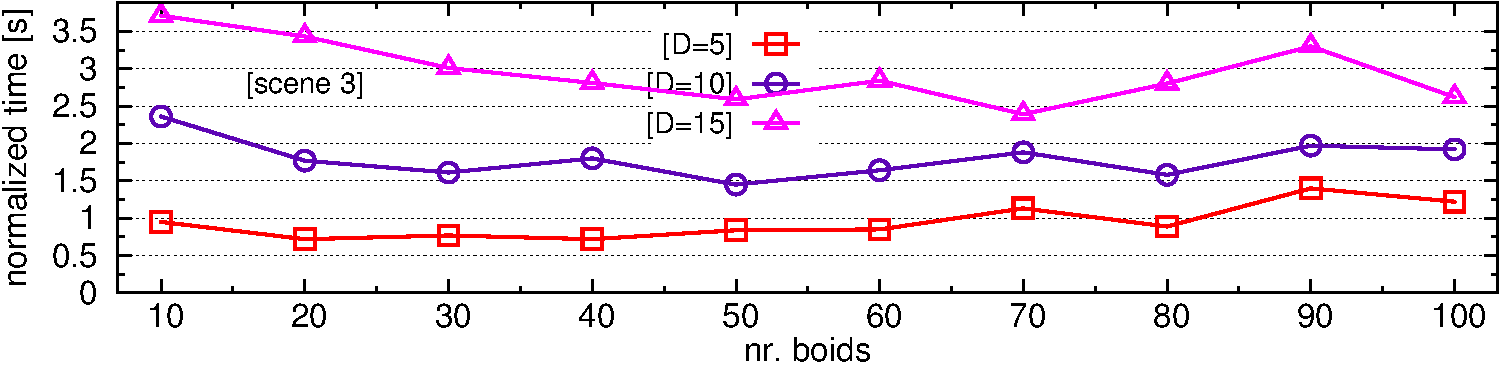
\includegraphics[width=\textwidth]{figs/figResScene3}
\caption{Results show the normalized median runtime as a function of
  the number of robots and the number of dynamic obstacles ($D =
  \{5,10,15\}$). Runtime is measured as the time from the beginning
  till the last robot reaches the goal. Normalization corresponds to dividing the median
  runtime by the number of boids. }
\label{fig:Res1}
\end{figure*}

\subsubsection{Measuring Performance}
A problem instance is defined by a scene, the number of robots, and
the number of dynamic obstacles. In the experiments, the number of
robots is varied from $10$ to $100$ in increments of $10$. The number
of dynamic obstacles is varied as $5, 10, 15$. Results for each
problem instance report median time based on ten different runs.
Experiments are conducted on an Intel Core i7 machine (CPU: 2 GHz,
RAM: 16GB) using OS X 10.9.1. Code is written in Python 2.7.3.

\subsection{Results}
\label{sec:Results}

Fig.~\ref{fig:Hist} provides a histogram on the percentage of robots
that reached the final goal during a particular time interval. The
figure illustrates that due to interference from dynamic obstacles
robots may reach the final goal at different times. As shown
next, $\Name$ is quite efficient and scales linearly with the number of
robots.

Fig.~\ref{fig:Res1} provides a summary of the results when varying both
the number of robots and the number of dynamic obstacles.  These results
show that $\Name$ is capable of efficiently enabling the swarm to
reach the final goal while avoiding collisions with static and dynamic
obstacles. As the
results indicate, $\Name$ scales linearly with the number of robots,
even as the number of dynamic obstacles is increased.

By combining roadmaps with potential fields, $\Name$ provides the
swarm with global path planning to guide toward the goal while
reacting to obstacles encountered along the way, making local
adjustment and seeking alternative pathways to avoid getting trapped. 
As such, branching plays a key role in the efficiency of
$\Name$. Fig.~\ref{fig:Branch1} provides a qualitative evaluation of
the impact of branching. As shown, without branching, robots have a
harder time finding a way around dynamic obstacles which prevent the
swarm from following the current pathway.


\begin{figure}
\centering
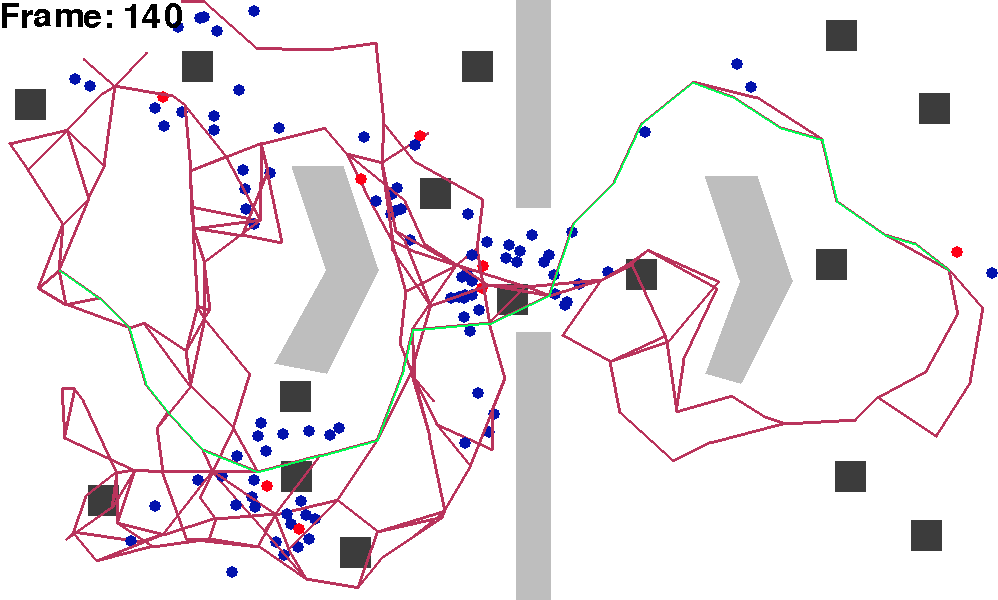
\includegraphics[width=0.23\textwidth,frame]{figs/hurdles_branching_1.png}
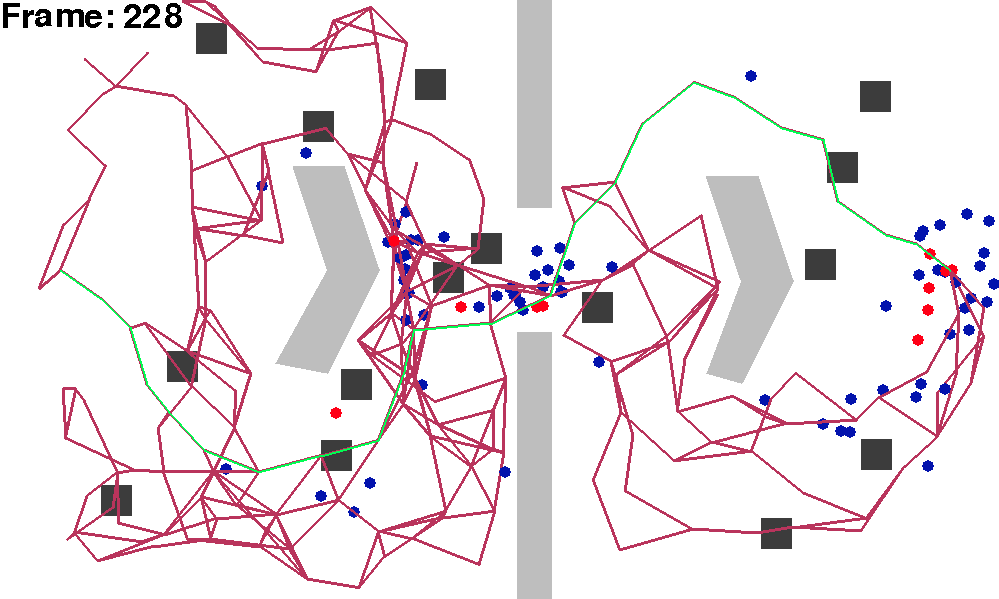
\includegraphics[width=0.23\textwidth,frame]{figs/hurdles_branching_2.png}\\
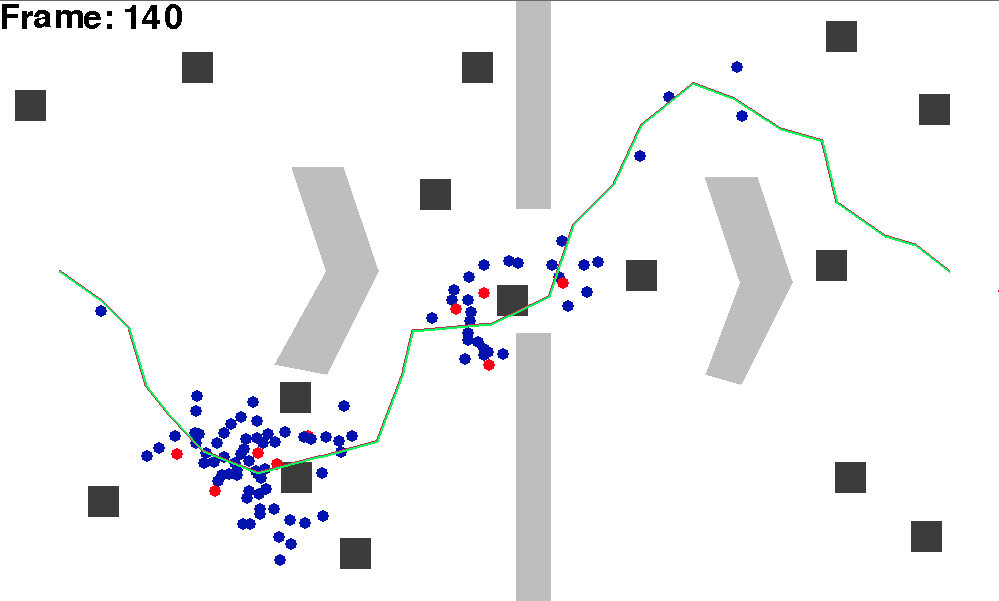
\includegraphics[width=0.23\textwidth,frame]{figs/hurdles_no_branching_1.png}
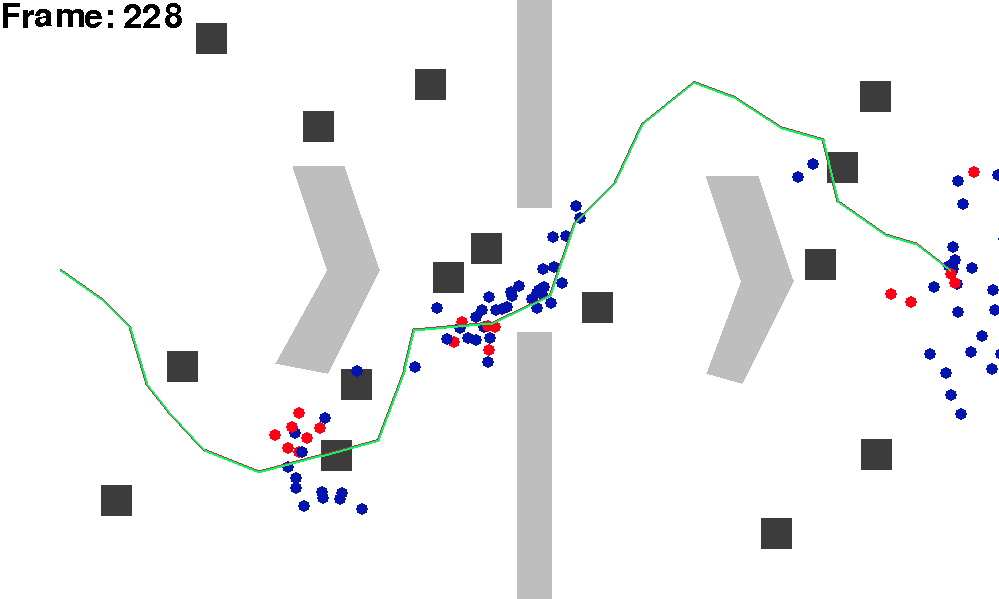
\includegraphics[width=0.23\textwidth,frame]{figs/hurdles_no_branching_2.png}
\caption{Qualitative comparison of $\Name$ with (top) branching enabled
  vs (bottom) branching disabled.}
\label{fig:Branch1}
\end{figure}

A quantitative comparison of the impact of branching is provided in
Table~\ref{table}.  The results show  that the time taken to navigate through
the environment when the branching is turned off is larger than the
time taken when the path branches. This is because of two
things. Firstly branching relieves the congestion around narrow
passageways and tries to split the swarm so it can ``move in
parallel.'' This means that instead of all of the robots going through
one passageway sequentially, two sets of swarms can go through
different paths at the same time. The second reason branching produces
better results is because the robots are not able to pre-generate a
shortest path that will always keep the swarm out of unrecoverable
configurations as they do not posses the ability to predict the
position of dynamic obstacles.  For example, if a dynamic obstacle
obstructs a narrow passageway and the shortest path goes through that
passageway, the robots will not be able to reach the end until the
obstacle moves out of the way if the path does not branch. However, if
the path branches, it is able to find a new way around the obstacle,
therefore avoiding the obstructed passageway. This reduces the amount
of time the swarm spends waiting and instead finds a new way to the
goal. This, of course, reduces the time it takes to get to the goal.


\begin{table}
\centering
\begin{tabular}{c|c|c|c}
\multicolumn{4}{c}{[scene 1 with 10 dynamic obstacles]}\\
 nr. robots   & 10    &  50 & 100\\\hline
 branching on & 10.87 & 26.14 & 73.83 \\
 branching off& 12.12 & 76.33 & 151.28 
\end{tabular}

\vspace*{2mm}

\begin{tabular}{c|c|c|c}
\multicolumn{4}{c}{[scene 2 with 100 robots]}\\
 nr. dynamic obstacles  & 5    &  10 & 15\\\hline
 branching on & 74.37 & 84.98 & 128.67 \\
 branching off& 141.59 & 138.09 & 231.57 
\end{tabular}

\caption{Impact of branching on $\Name$. Results show median time
  when enabling or disabling branching in $\Name$}
\label{table}
\end{table}





\section{Discussion}

This paper proposed $\Name$, a path-planning approach to enable a
swarm of robots move to a goal region while avoiding collisions with
static and dynamic obstacles. Scalability is obtained by an efficient
combination of probabilistic roadmaps to provide global path planning
with potential fields to provide local, reactive, behaviors necessary
to avoid collisions with obstacles. A key component of $\Name$ is the
branching aspect which provides alternative pathways to help stuck
robots successfully find their way to the goal. Experimental results
with an increasing number of robots and numerous dynamic obstacles
show the efficiency and scalability of the approach.  For future work,
one direction is to predict the motions of dynamic obstacles and
incorporate those predictions to adjust the roadmap so that it can
provide alternative pathways that avoid predicted
trajectories. Improving the roadmap quality may also improve the
overall performance of $\Name$. Another direction is to make use of
high-level formation behaviors that can be leveraged to more easily
move through certain narrow passages.

\bibliographystyle{IEEEtran} 
\bibliography{mp,plaku}


\end{document}

